\documentclass[../../../main.tex]{subfiles}

\begin{document}

Whittier College prides itself on doing right by our diverse student body.  In Sec. \ref{sec:teaching_philosophy}, I shared my reflections on the place physics holds within the liberal arts perspective.  What I did not share in that section was that STEM courses are not known for being diverse, nor for fostering equity and inclusion\footnote{This is particularly pronounced for the topic of gender, although explaining that nuanced situation is outside my level of expertise and beyond the scope of this report.}.  What might come as a surprise is that many STEM professors work diligently to foster equity and inclusion in their classes, often unnoticed.  In Sec. \ref{sec:oer}, I reflect on student utilization of open educational resources (OER).  In Sec. \ref{sec:arrange}, I reflect on my experience with flexibility for students with a wide range of issues during the pandemic.  Finally, in Sec. \ref{sec:cec}, I reflect upon our experience with the Artemis program under the Center for Engagement with Communities (CEC).

\subsection{Open Educational Resources (OER)}
\label{sec:oer}

I have given several lectures before and during the pandemic at OER workshops organized by Sonia Chaidez and Azeem Khan\footnote{I have included my slides for those lectures in the supplemental material.}.  Wardman staff conducted focus groups, and the results were similar to those of other institutions.  About 1 in 5 students have difficulty buying books.  Further, some students cannot justify spending precious extra dollars on books when the professor only covers half the content within them.  To address this problem, my students and I use OpenStax resources in all courses for which that is possible\footnote{There is a growing library of texts in areas beyond STEM.  See \url{https://openstax.org} for more information.}.  Without a homework system, professors of physics at Whittier College could spend 15-20 hours per week grading just homework.  My colleagues and I have used a service called TheExpertTA that administers and grades homework while charging the student \$32.50.  I'm pleased to share with you that during Spring 2021, my students and I learned to use OpenStax Tutor, the homework system fully integrated with OpenStax textbooks.
\\
\vspace{0.25cm}
OpenStax Tutor costs the students only \$10.00, and the books are free.  Tutor adds several key features beyond TheExpertTA.  First, \textit{reading assignments} can be created to incentivize the students to finish the reading before class.  Second, the homework problems can be multiple choice, conceptual, or require a longer calculation.  That adds flexibility for our students, as some learn at a faster or slower pace.  Third, the OpenStax Tutor system uses machine learning to determine the concepts that cause an individual student to struggle, and assigns them customized practice problems.  I receive statistical reports, and I act on them by covering those exercises in class with which many students struggled.  Finally, the system summarizes the reading and homework schedule for the students in a calendar and notification system.  Figure \ref{fig:openstax} gives an example of this.  In summary, the system is more adaptable, more feature-rich, and more cost-effective for our students.  Table \ref{tab:oer} contains a list of all courses I have taught in my time at Whittier College, and includes the use of OER.
\\
\vspace{0.25cm}

\begin{figure}
\centering
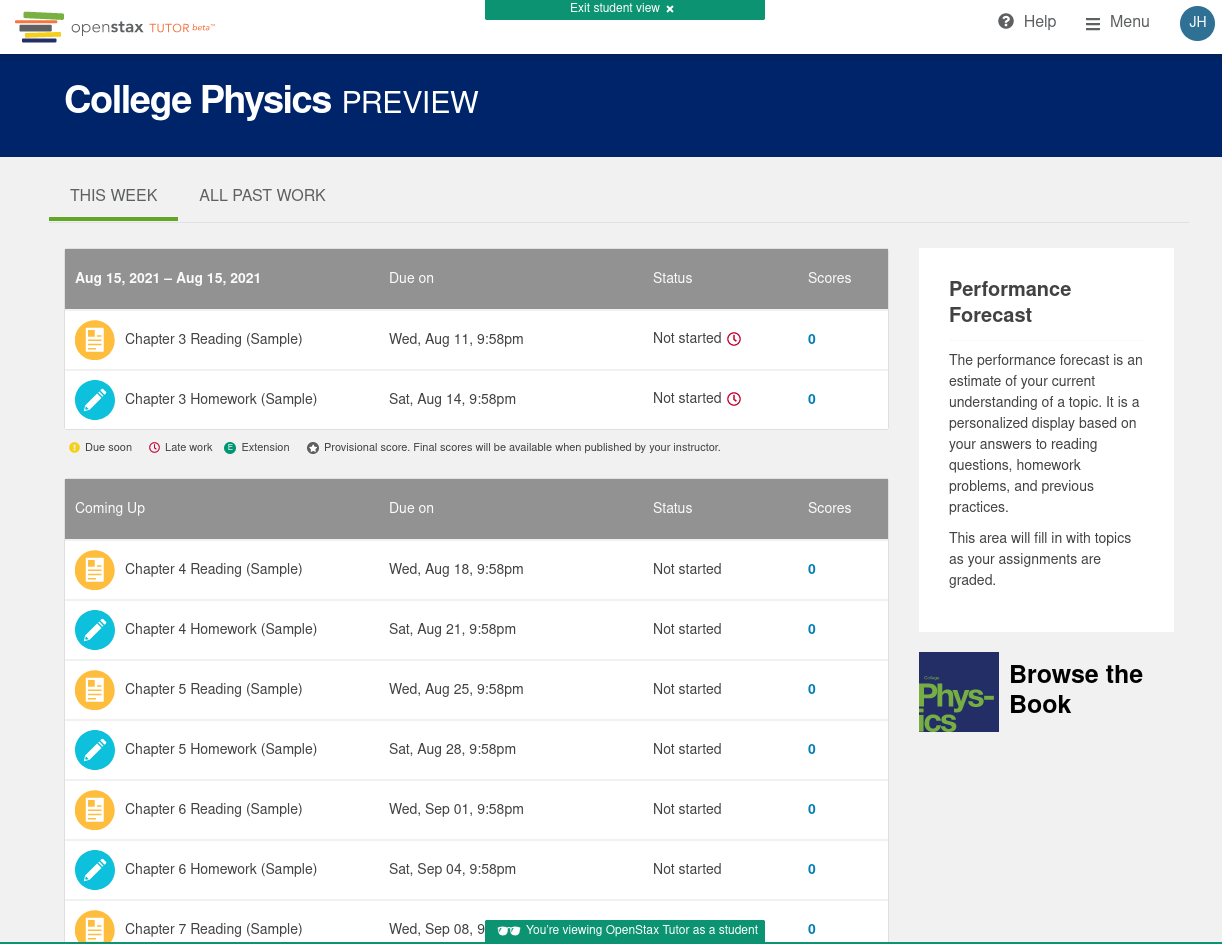
\includegraphics[width=0.4\textwidth]{figures/openstax1.png}
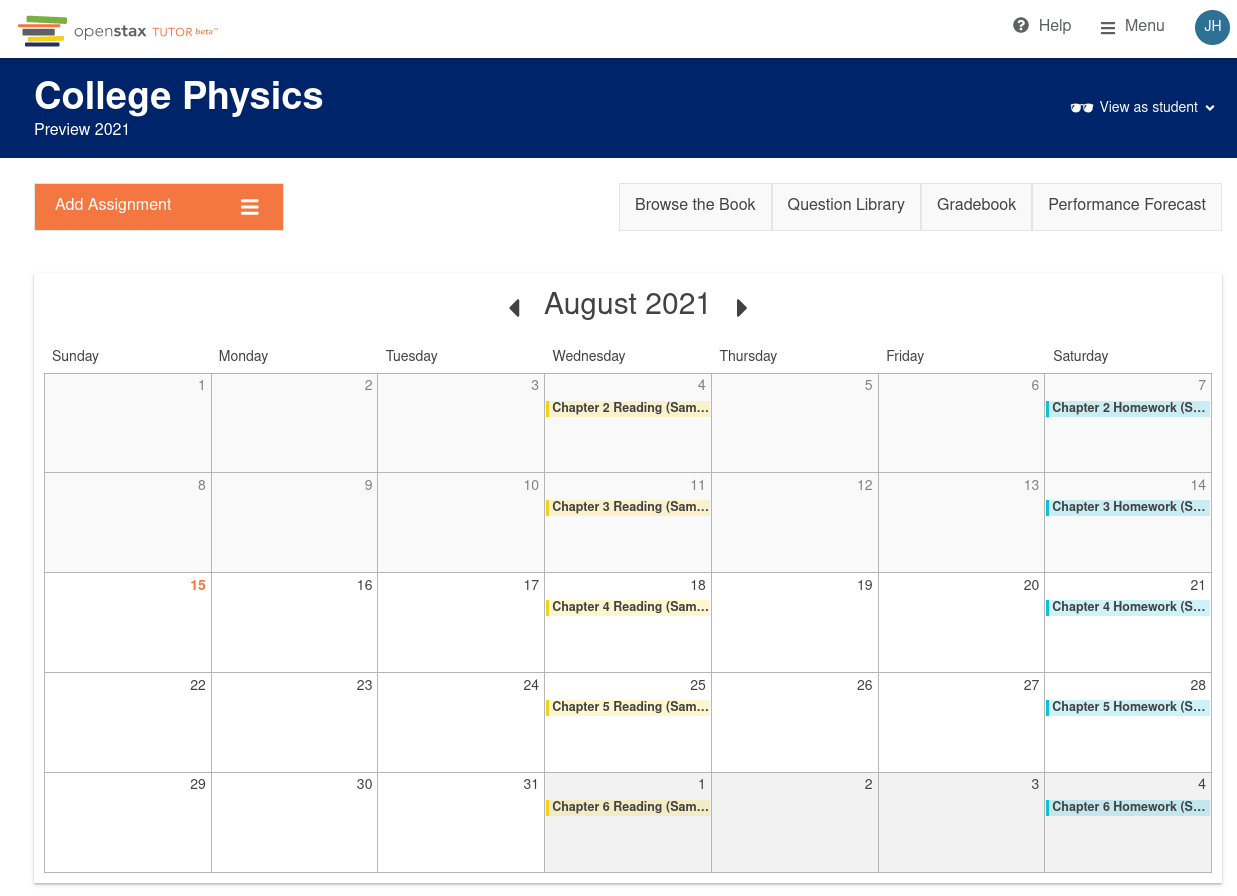
\includegraphics[width=0.4\textwidth]{figures/openstax2.png}
\caption{\label{fig:openstax} (Left) Student view of OpenStax Tutor.  (Right) Professor view.  In both pictures, reading assignments are in yellow and homework assignments are in blue.}
\end{figure}

\begin{table}
\small
\centering
\begin{tabular}{| c | c | c | c | c | c |}
\hline \hline
Semester & Course & Credits & Students & Curriculum feature & OER Usage\\ \hline
Fall 2017 & PHYS135A-01 & 4.0 & 24 & Intro & OpenStax \\ \hline
Fall 2017 & PHYS150-01 & 4.0 & 17 & COM1/Intro & OpenStax \\ \hline
Spring 2018 & PHYS135B-01 & 4.0 & 18 & Intro & OpenStax \\ \hline
Spring 2018 & PHYS180-02 & 5.0 & 19 & COM1/Intro & OpenStax \\ \hline
Spring 2018 & COSC330/PHYS306 & 3.0 & 6 & Advanced & PYNQ-Z1 \\ \hline
Fall 2018 & PHYS135A-01 & 4.0 & 24 & Intro & OpenStax \\ \hline
Fall 2018 & PHYS135A-02 & 4.0 & 26 & Intro & OpenStax \\ \hline
Jan 2019 & COSC390 & 3.0 & 8 & Advanced & open-access text \\ \hline
Spring 2019 & PHYS135B-01 & 4.0 & 25 & Intro & OpenStax \\ \hline
Spring 2019 & PHYS180-02 & 4.0 & 9 & Intro/COM1 & OpenStax \\ \hline
Fall 2019 & PHYS135A-01 & 4.0 & 24 & Intro & OpenStax \\ \hline
Fall 2019 & PHYS150-02/03 & 4.0 & 26 & COM1/Intro & OpenStax \\ \hline
Fall 2019 & INTD255 & 3.0 & 23 & CON2 & OPS \\ \hline
Spring 2020 & COSC330/PHYS306 & 3.0 & 13 & Advanced & PYNQ-Z1 \\ \hline
Spring 2020 & PHYS135B-01 & 4.0 & 23 & Intro & OpenStax \\ \hline
Spring 2020 & PHYS180-02 & 4.0 & 24 & COM1/Intro & OpenStax \\ \hline
Fall 2020 (Module 1) & INTD100-21 & 3.0 & 14 & Intro & -- \\ \hline
Fall 2020 (Module 2) & PHYS330 & 3.0 & 11 & Advanced & -- \\ \hline
Spring 2021 (Module 1) & INTD290 & 3.0 & 26 & CON2,CUL3 & WeVideo \\ \hline
Spring 2021 (Module 2) & PHYS135B-02 & 4.0 & 17 & Intro & OpenStax/Tutor \\ \hline
Spring 2021 (Module 3) & PHYS135B-01 & 4.0 & 25 & Intro & OpenStax/Tutor \\ \hline
-- & Total & 78.0 & -- & -- & -- \\ \hline \hline
Summer 2020 (Session II) & MATH080 & 3.0 & 11 & Intro & OpenStax \\ \hline
\hline
\end{tabular}
\caption{\label{tab:oer} This table is a summary of courses taught in four years, plus Summer sessions.  Not included: PHYS396 (Physics Research for Credit), and PHYS499 (Senior Seminar).  OpenStax and OpenStax Tutor are examples of OER in STEM.  The PYNQ-Z1 is a circuit board integrated with open-source software.  WeVideo is a web-based video editing platform.  OPS stands for Open Polar Server.}
\end{table}

Open Educational Resources were also used in my advanced and liberal arts courses.  In Computer Logic and Digital Circuit Design (COSC330/PHYS306), students design digital electronics on an integrated circuit board called the PYNQ-Z1 by Agilent (\url{https://www.pynq.io}).  The Python3 software the students use to operate this device is open-source, and our department purchased the boards and laptops to go with them.  There is zero cost to the student.  In Digital Signal Processing (DSP), COSC390, the text is open-access and the course software is written by me in octave, an open-source programming language the students install for free.  In INTD255, the course about Antarctic science, the students use the Open Polar Server (OPS) to access data about ice sheets and ice shelves around the world for climate science purposes.  In INTD290, the course about Latin American science, students used WeVideo to create digital storytelling projects.  Whittier College has a site license for WeVideo, at no cost to the students.

\subsection{Making Arrangements for a Diverse Group of Students}
\label{sec:arrange}

Even before the pandemic, my students faced time-pressures.  I observed how non-majors and introductory students took exams.  The grading data revealed that most students would do well on homework but midterms and final exams caused some problems.  Typically three-fourths of my students are KNS or Biology majors, who are \textit{required} to take algebra-based physics (PHYS135A/B).  They are also required to take courses like organic chemistry.  When midterms in these courses coincide with my midterms, we have difficulties.  I shifted away from a rigid testing schedule, and polled the students regarding the optimal date for midterms.  The students really appreciated that, and I began to write take-home exam versions in case a student had to travel for sports or family on the day the class selected.  The students appreciate flexibility, expecially when they work or care for family.
\\
\vspace{0.25cm}
The flexibility techniques I was learning in 2019-2020 had to be turbo-charged for the module system and remote instruction.  I learned about the Calendly booking service from an Wardman Library workshop.  This taught me what a booking service is, and I quickly located a free version: \url{https://10to8.com}.  The software synced with my calendar and provided a convenient booking page for the students (like a doctor's office).  I ensured that my students could grab 30 minutes of my time when they were free.  For example, I met with students while they were on break at work via Zoom to go over homework.  Because the homework and book are open-access, the could see all course content.
\\
\vspace{0.25cm}
My physics courses usually involve a student-designed final project.  In my early years at Whittier College, I noticed some students would create sophisticated projects using our lab equipment, and some would create them at home with household items.  I could have jettisoned that part of my syllabus during remote instruction, given that the students had no access to our labs.  However, the students really shine when designing and executing their own ideas.  I decided it would boost inclusivity by allowing the students to demonstrate their projects for each other via Zoom, and to cheer for each other.  Some students even presented DIY Arduino integrated circuits, similar to my students in the Artemis program.

\subsection{Center for Engagement with Communities: Artemis Program}
\label{sec:cec}

According to a demographic study done by the American Institute of Physics (AIP), women earned about 20\% of bachelor's degrees and doctorates in physics in 2017 \cite{aip}.  The overall graduate student enrollment has fluctuated around 3000 people in the United States in the decades prior to the release of the AIP report.  This implies that there are only $\approx 600$ women signed up to earn a PhD in physics in the USA \textit{per year.}  I remarked earlier in a footnote that this is a complex, multi-faceted issue with many variables not under my control.  However, there are ways in which I can help foster inclusion in STEM at Whittier College.
\\
\vspace{0.25cm}
In Fall 2018, Prof. Serkan Zorba and a program coordinator with the Center for Engagement with Communities (CEC) named Samantha Ruiz approached me about joining the Artemis Program.  The Artemis Program fosters inclusion by inviting young ladies from local high schools to learn about Whittier College.  They perform research with Whittier College professors, and CEC staff help them with the Whittier College application.  I answered the call to serve, and began designing a Python3-based physics education project.  This experience tested my teaching ability.  I had to establish \textit{order} creatively (Sec. \ref{sec:teaching_philosophy}), and asked the girls to write code together (\textit{shared meaning}).  They eventually presented their results at URSCA 2019, after they wrote Python3 code that gathered data about how quickly and accurately their fellow high school students solved physics problems.
\\
\vspace{0.25cm}
In Spring 2020, I served the Artemis Program a second time.  My idea was for the young ladies to create wearable Arduino circuit boards that would connect to WiFi.  The purpose was to relay location information in case an elderly loved one got lost.  I began with demonstrations and code examples, and eventually the girls got their boards to communicate via WiFi.  Before we could work on making the little boards \textit{wearable}, the pandemic struck and URSCA was cancelled.  Nevertheless, the young ladies got to keep their boards and continue developing at home.  I look forward to seeing some of them again this Fall.

\end{document}
